\section{Architectural Design}
\subsection{Overview}
	The main architecture chosen for this system is the client-server one; clients access the service through the web server that is only the view of the system. 
	
	All services are inside the application server that exposes all the APIs needed to expand the system in the future.
	
	All the data is stored inside a database that is on another machine.

	This modular schema helps the system maintainability because every component is independent from the other and they can be substituted without replacing other parts. 
\subsection{High level components and their interaction}
	Starting from the user or taxi, every request is made to the web server that can serve all the static pages which contain only the basic structure and the graphics of the website. Every type of user can access only his interface:
	\begin{itemize} 
		\item taxis can access their interfaces to manage their rides 
		\item users can access only the reservation interfaces where they can make a new reservation or modify/delete one.
	\end{itemize}
	To populate all the pages with the needed data, the web server needs to ask the application server.
	
	The application server receives and elaborates the request: if there is the necessity, it will query the database server to retrieve or save the needed data for the request.
	
	The database server stores all the data received from the application server and it waits for queries.
\subsection{Component view}
	\begin{center}
		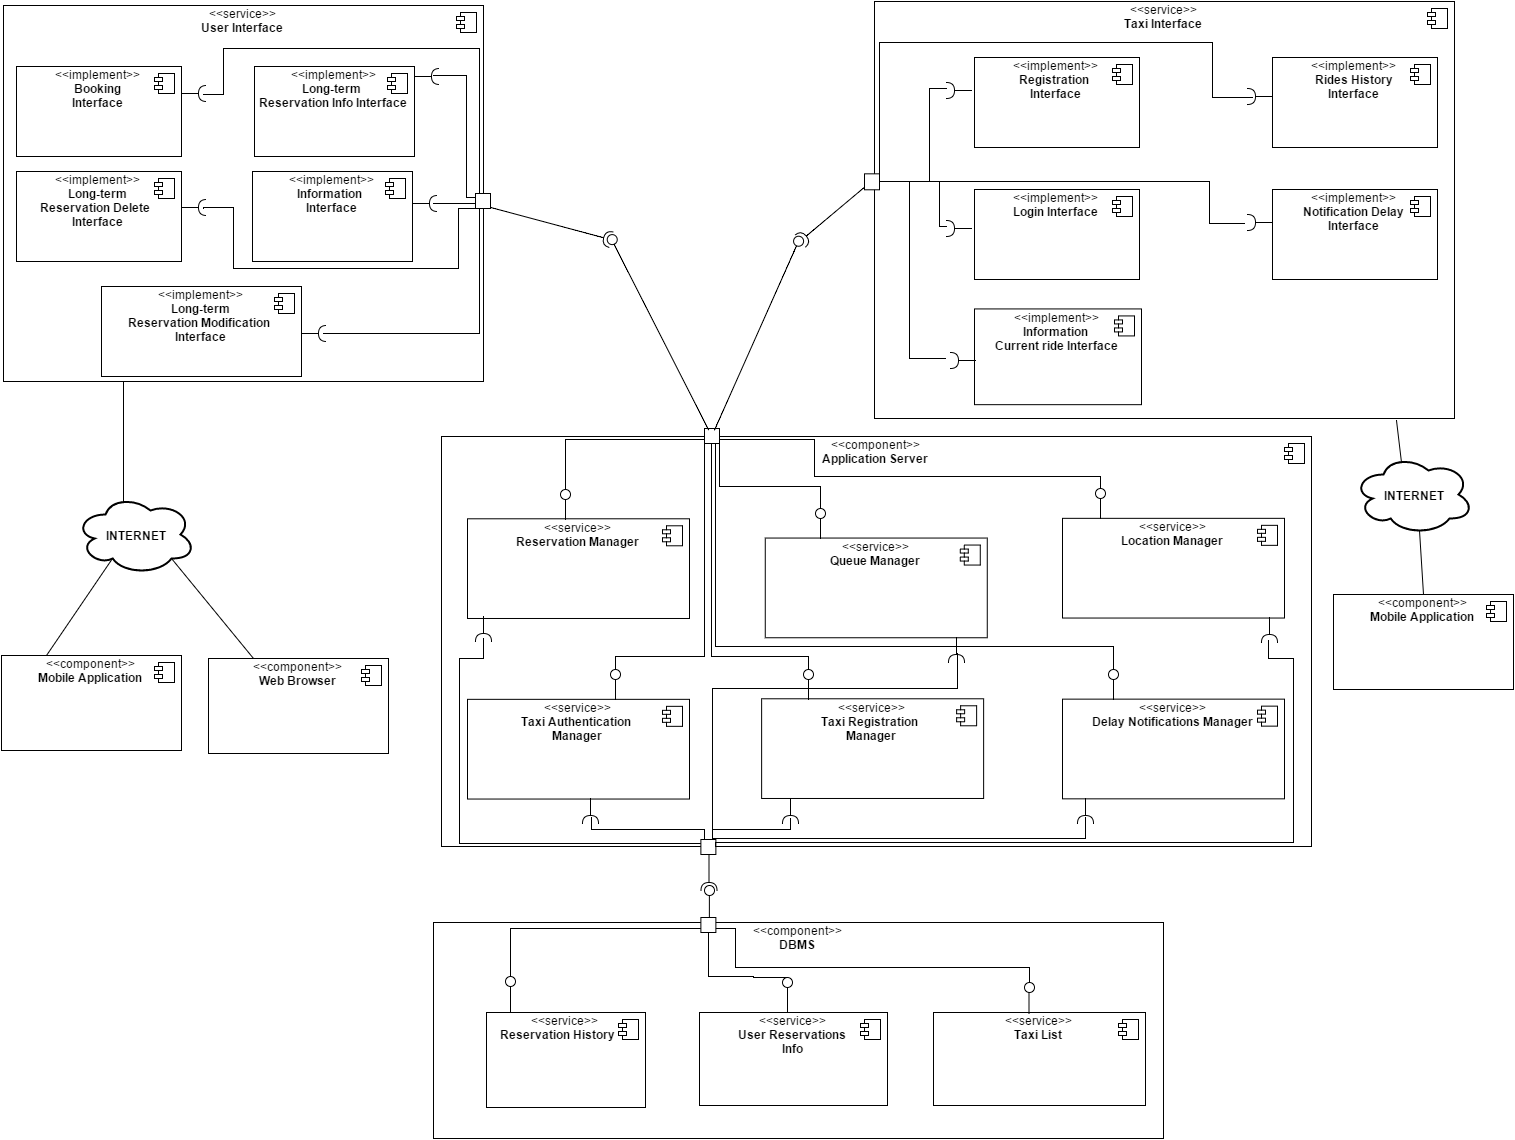
\includegraphics[width=0.95\textwidth]{./images/component_view.png}
	\end{center}
	
	In the above diagram, through the Internet, using a web browser or, in alternative, a smartphone, users can access to their interfaces, that are about the booking, the modification of the long-term reservation, the long-term reservation information, the service information and the elimination of the long-term reservation. 
	
	In the case of taxis, through the Internet, only using a smartphone, they can access to their interfaces, that are about the registration, the history of the rides, the login, the notifications of delay and the information about the current ride.
	
	These interfaces are populated with data, coming from the application server. This is composed of some services that manage the reservations, the queues of taxis, the locations of the users, the taxis' authentication, the taxis' registration and finally the delay' notifications.
	
	The application server is the only component that can access to the DBMS, which is characterized by three data tables: the history of the reservations, the users' reservations and the taxis' list.
\subsection{Deployment view}
	\begin{center}
		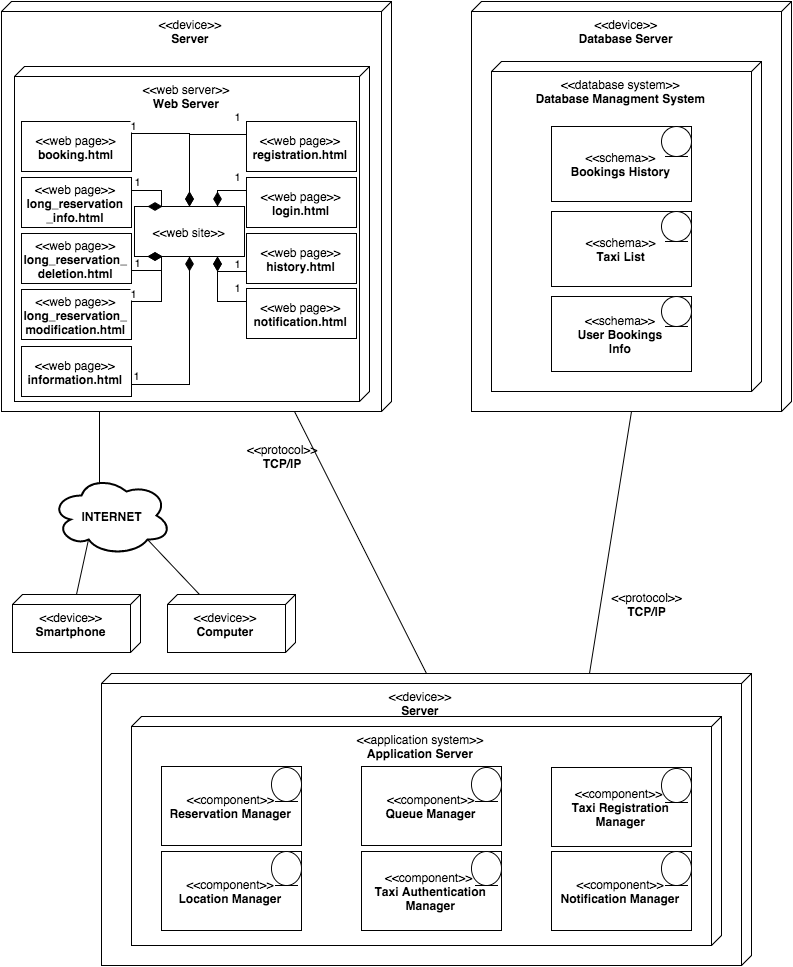
\includegraphics[width=0.95\textwidth]{./images/deployment_view.png}
	\end{center}
	
	In the above diagram, through the Internet, using a web browser and/or a smartphone, users and taxis can access to the server, which contains the web server. Here, there are some pages that represent which stuff, clarified in the component view description, a user or a taxi can do.
	
	Thanks to the TCP/IP protocol, the server of the web one is connected to the application server: it contains all the application logic, that lets to the pages of the web server to be populated with data.
	
	This application system is composed by the same managers, clarified in the component view description.
	
	Finally, the server of the application one is linked, thanks to the TCP/IP protocol, to the database server: through this connection, the application server communicates to the web server the data from the database, which contains the same three tables, clarified in the component view description. 

\subsection{Runtime view}
	\subsubsection{Taxi Registration}
		Taxi registration is fully described in RASD section \textbf{3.5.2}
		\begin{center}
			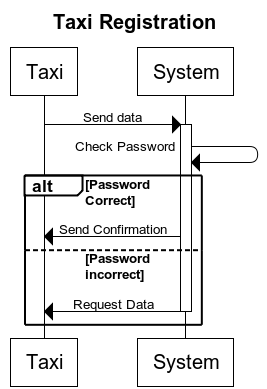
\includegraphics[width=0.70\textwidth]{./images/Taxi_Registration.png}
		\end{center}
	\subsubsection{Short Term Reservation}
		\begin{center}
			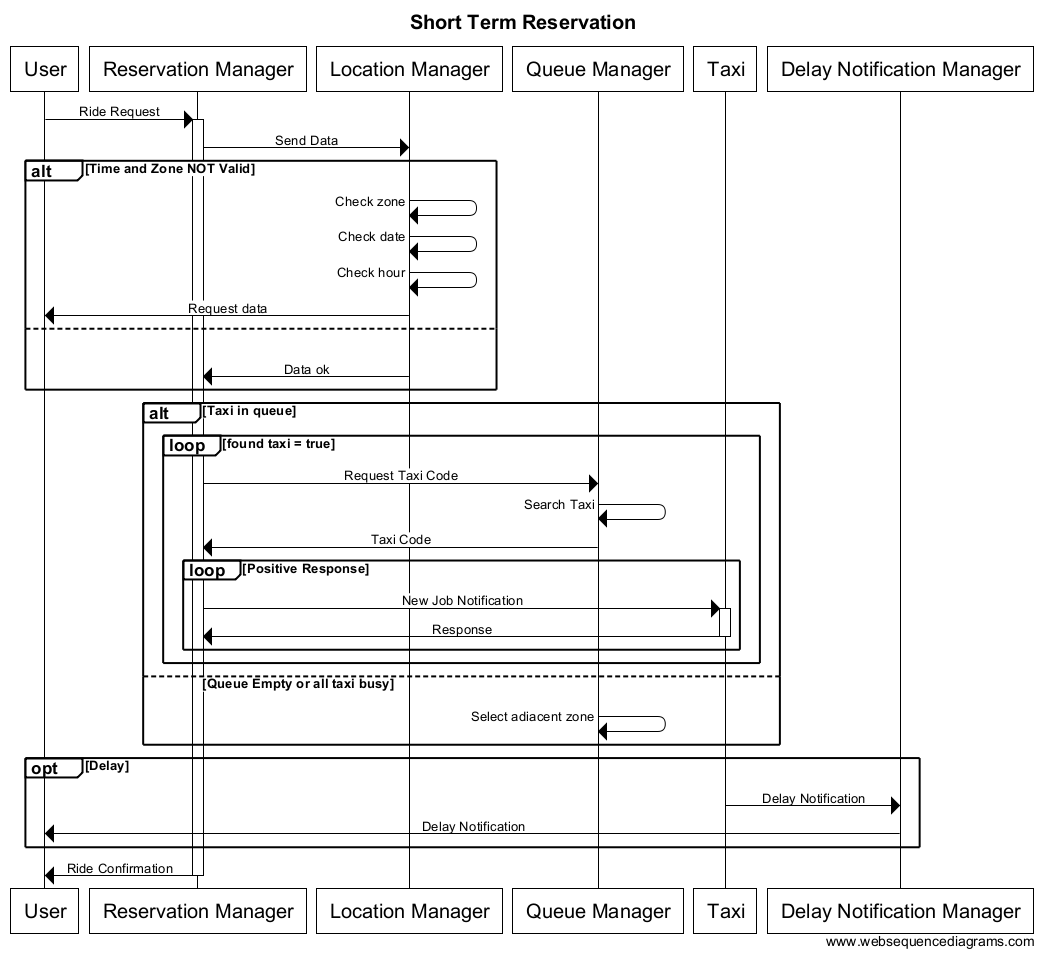
\includegraphics[width=0.85\textwidth]{./images/Short_Term_Reservation_Complete.png}
		\end{center}
	\subsubsection{Long Term Reservation}
		\begin{center}
			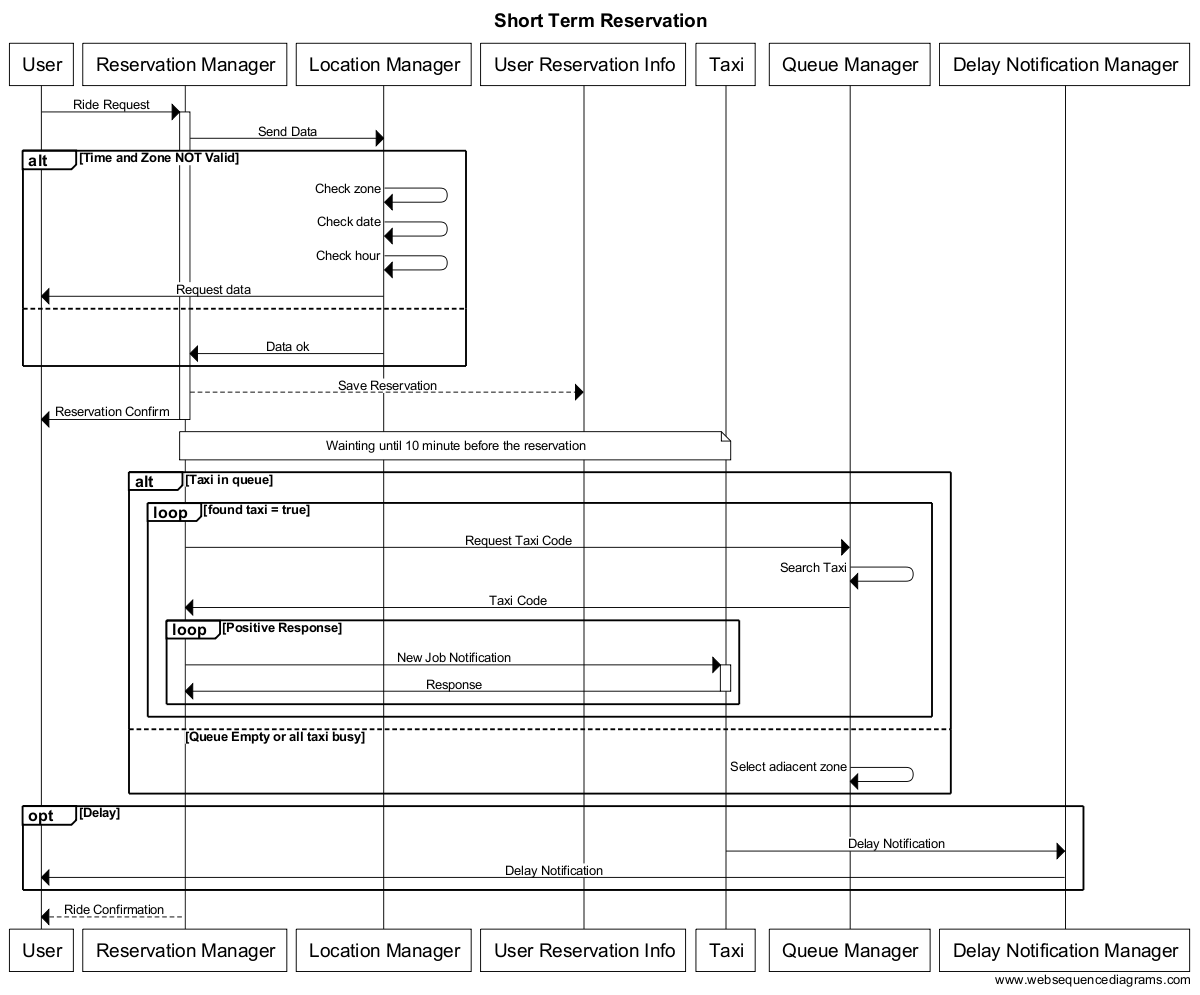
\includegraphics[width=0.85\textwidth]{./images/Long_Term_Reservation_Complete.png}
		\end{center}
\subsection{Component interfaces}
	Every part of the system provides a specific interface to interact with the other parts; in particular the system has:
	\begin{itemize}
		\item \textbf{Website Interface:} This interface is used by the clients in order to display the web pages provided by the web server.
		\item \textbf{Application Server Interfaces:} These interfaces are used by the web server to query the application server for the data that is needed in the web pages. Every manager in the application server has its own interface in order to keep, as much modular as possible, the application server in order to make it easier, to scale up it with more services.
		\item \textbf{Database Interface:} This interface provided by the database allows to query or modify the database by the application server. Since this is the only interface provided by the database, only the application server can access it, providing data security.
		\item \textbf{Application Programming Interfaces:} These interfaces allow the system to be upgraded and expanded with new functionalities.
	\end{itemize}
\subsection{Selected architectural styles and patterns}
	The system is organized with a Client-Server architecture, but the application server is divided in several managers which manage every service. 
	
	The GUI part of the system are the cellphones and the website that allow the users and the taxis to access the system through the internet network.
	
	The figure on the left shows a system that has the application server and the database in the same place and it don't need any network connection between them. The figure on the right instead shows how the system can be distributed and it can be scaled more easily.
	\begin{center}
	    \begingroup
	    	\setlength{\tabcolsep}{30pt}
		    	\begin{tabular}{ c | c }
			    	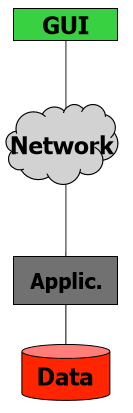
\includegraphics[width=0.10\textwidth]{./images/architecture1.png} & 	
			    	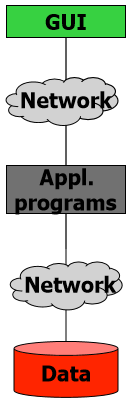
\includegraphics[width=0.10\textwidth]{./images/architecture2.png}  \\ 
		    	\end{tabular} 
	    	\end{center}
		\endgroup
	\end{center}	  	
\subsection{Other design decisions}
	\subsubsection{Design patterns}